\chapter{Fundamentação teórica}
\section{Sistemas de Referência}

Definir posições de um objeto ou alvo de estudo sobre a superfície terrestre requer um tratamento matemático \cite{d1999coordenadas}, a fim de estabelecer a localização em relação a uma origem. Os sistemas de coordenadas são definidos em termos da orientação, métrica e curvatura \cite{torge2001geodesy}. Dentre os sistemas de referência abordados na literatura, cuja nomenclatura pode ser distinta daquela apresentada neste estudo, destacam-se três que são os mais utilizados em geofísica aplicada. Todos eles seguem o movimento de rotação da Terra e são utilizados na descrição matemática das posições de objetos localizados sobre ou próximos à superfície terrestre \cite{torge}.

O \textit{Sistema Cartesiano Geocêntrico} $(SCG)$ faz uso do sistema de coordenadas ortogonais $\mathbf{XYZ}$, cuja origem coincide com o centro de massa da Terra. O eixo $\mathbf{Z}$ coincide com o eixo de rotação médio da Terra e, portanto, aponta para o polo norte, $\mathbf{X}$ aponta na direção  do meridiano médio de \textit{Greenwich} e $\mathbf{Y}$ é o eixo complementar segundo a regra da mão direita \cite{soler1976differential,soler1988,torge}, como exemplificado na Figura~\ref{fig:datum}.a.

O \textit{Sistema Geodésico Geocêntrico} (SGG) é largamente utilizado em sistemas de navegação por GPS (\textit{Global Positioning System}, \cite{cai2011}) e é definido de acordo com um modelo de elipsoide de referência usado para representar a Terra Normal. Este elipsoide é estabelecido uma vez que são fixados, principalmente, os semieixos maior e menor, $a$ e $b$, respectivamente, conservando, assim, o achatamento terrestre $(f)$ nos polos. Nesse sistema, a origem está localizada no centro do elipsoide de referência \cite{soler1976differential} e um ponto fictício $P$ na superfície terrestre é posicionado a partir de três coordenadas: altitude geométrica ($h$), que corresponde à distância do ponto $P$ à superfície  do elipsoide, medido na direção normal àquele; a latitude geodésica ($\varphi$), que é definida como o ângulo que a \textit{normal} ao elipsoide  forma com sua projeção equatorial; a longitude ($\lambda$), que é o ângulo diedro formado pelo meridiano de Greenwich e o meridiano passante pelo ponto $P$ como pode ser visto nas Figuras~\ref{fig:datum}.a e ~\ref{fig:datum}.b. Para cada ponto $(h,\varphi,\lambda)$, existem três vetores unitários ortogonais entre si, formando os eixos do sistema de coordenadas, definidos por \citeonline{soler1976differential}:

\begin{equation}
\label{eq:vetores_unitarios}
\displaystyle \mathbf{\hat{u}} = 
\left(\begin{array}{c}
\cos{\varphi} \cos{\lambda} \\ \cos{\lambda} \sin{\lambda}\\  \sin{\varphi}
\end{array} \right)  \quad ; \quad
\mathbf{\hat{v}} =
\left(\begin{array}{c}
-\sin{\varphi} \cos{\lambda} \\ -\sin{\varphi} \sin{\lambda} \\ \cos{\varphi}
\end{array} \right)  \quad ; \quad
\mathbf{\hat{w}} =
\left(\begin{array}{c}
-\sin{\lambda} \\ \cos{\lambda} \\ 0
\end{array} \right)
\end{equation} 

\begin{figure}[h]
	\centering
	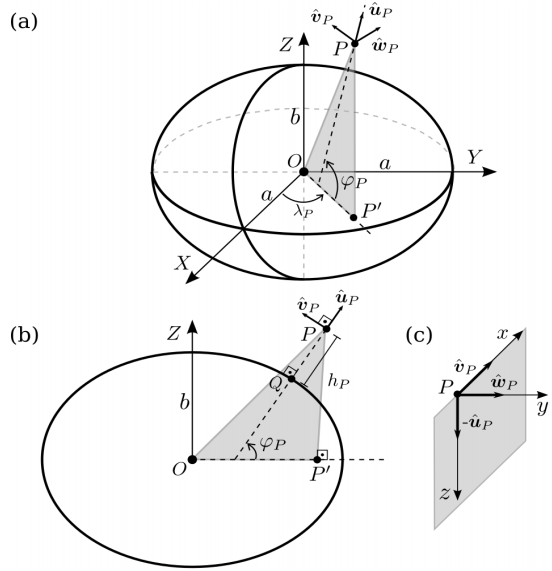
\includegraphics[width=10cm,height=10cm]{figs/sistemas_de_referencia.png}
	\caption{ (a) e (b) são Sistema Cartesiano Geocêntrico ($SCG$) e Sistema Geodésico Geocêntrico ($SGG$), respectivamente. A posição de um ponto no $SCG$ é definida pelas coordenadas cartesianas geocêntricas ($X,Y,Z$), em que o eixo $Z$ coincide com o eixo médio de rotação da Terra, o eixo $X$ aponta para o Meridiano de Greenwich e o eixo $Y$ aponta para leste. O $SGG$ é definido por um esferoide oblato com semieixo maior $a$ e semieixo menor $b$. Neste sistema, a posição de um ponto é determinada pelas coordenadas geodésicas: altitude geométrica ($h$), latitude geodésica ($\varphi$) e longitude ($\lambda$). Os vetores unitários \textbf{û}, $\mathbf{\hat{v}}$ e \textbf{ŵ} definem direções ortogonais, em um determinado ponto. As quantidades associadas ao ponto $P$ estão indicadas com o subscrito $P$. Em (b), $Q$ representa um ponto sobre o elipsoide de referência na mesma latitude e longitude do ponto $P$. (c) é o Sistema Cartesiano Topocêntrico ($SCT$) com origem em um ponto $P$. Nesse sistema, a posição de um ponto é definida por coordenadas cartesianas topocêntricas ($x,y,z$) em que $x$ e $y$ são paralelos aos vetores unitários $\mathbf{\hat{v}}$ e \textbf{ŵ}, respectivamente, e o eixo $z$ é oposto a \textbf{û}. Em (c), o $SCT$ é representado com origem no ponto $P$. O plano de cor cinza é o mesmo mostrado em (a) e (b). Retirado de \citeonline{kristoffer}.}
	\label{fig:datum}
\end{figure}

Estudos geodésicos apresentam valores levemente diferentes para os parâmetros  $a$, $b$, $f$ e a excentricidade $e$ do elipsoide. Assim, ao utilizar o $SGG$, cada região do planeta deve adotar como referência o elipsoide mais adequado. A tabela~\ref{tab:ref_ellip} exemplifica alguns dos elipsoides de referência encontrados na literatura. No Brasil, é recorrente o uso do \textit{Sistema de Referência Geocêntrico para as Américas 2000} (SIRGAS2000) e do \textit{World Geodetic System} 1984 (WGS84). Este último foi o elipsoide adotado para este trabalho, uma vez que, é o sistema adotado pela base de dados do ICGEM.

\begin{table}[]
	\caption {Modelos de elipsoide de referência \cite{li2001}, \url{https://microem.ru/files/2012/08/GPS.G1-X-00006.pdf}} \label{tab:ref_ellip} 
	\centering
	\begin{tabular}{c|c|c|c|c}
		Modelo & a & b & 1/f \\
		\hline
		Airy                  & 6377563.396 & 6356256.909 & 299.324965 \\ \hline 
		Australian National   & 6378160.000 & 6356774.719 & 298.250000 \\ \hline
		Bessel 1841 (Namibia) & 6377483.865 & 6356165.383 & 299.152813 \\ \hline
		Clarke 1880           & 6378249.145 & 6356514.870 & 293.465000 \\ \hline
		Everest 1969          & 6377295.664 & 6356094.668 & 300.801700 \\ \hline
		Fischer 1968          & 6378150.000 & 6356768.337 & 298.300000 \\ \hline
		International         & 6378388.000 & 6356911.946 & 297.000000 \\ \hline
		Krassovsky            & 6378245.000 & 6356863.019 & 298.300000 \\ \hline
		SGS 85                & 6378136.000 & 6356751.302 & 298.257000 \\ \hline
		SIRGAS 2000           & 6378137.000 & 6356752.314 & 298.257222 \\ \hline
		South American 1969   & 6378160.000 & 6356774.719 & 298.250000 \\ \hline
		WGS 60                & 6378165.000 & 6356783.287 & 298.300000 \\ \hline
		WGS 66                & 6378145.000 & 6356759.769 & 298.250000 \\ \hline
		WGS 72                & 6378135.000 & 6356750.520 & 298.260000 \\ \hline
		WGS 84                & 6378137.000 & 6356752.314 & 298.257224 \\ \hline
	\end{tabular}
\end{table}

O \textit{Sistema Cartesiano Topocêntrico} $(SCT)$ é utilizado para estudos de escala local e regional. Ele tem relação direta com a superfície terrestre, já que é sobre ela que se posiciona a origem do sistema \cite{cai2011}, escolhida convenientemente. Sendo assim,  seus eixos $\mathbf{x}$ e $\mathbf{y}$ são definidos pelos mesmos vetores unitários $\mathbf{v}$ e $ \textbf{w}$ da equação \ref{eq:vetores_unitarios} que apontam para o norte e leste geográfico, respectivamente. O eixo $\mathbf{z}$, por outro lado, é definido pelo vetor que possui mesmo módulo e mesma direção de $\textbf{u}$ porém com sentido contrário, direcionado para dentro da Terra e ao longo da normal do elipsoide \cite{cai2011}, de acordo com a Figura \ref{fig:datum}.c.

A escolha de um sistema de coordenadas depende de sua simplicidade e eficácia com relação ao trabalho em questão. Enquanto aplicações globais exigem sistemas de coordenadas geocêntricos, para problemas de extensão limitada, sistemas de coordenadas locais ou topocêntricos bastam \cite{torge2001geodesy}.

\section{Potencial de Gravidade}
Começamos esta seção destacando o conceito primordial para a compreensão de todas as etapas deste trabalho: o conceito de função potencial e a sua definição associada à aceleração da gravidade. O conceito de potencial está associado ao trabalho realizado por uma força sobre um corpo ou partícula imerso(a) em um campo vetorial de forma a deslocá-lo(a). O trabalho considerado neste contexto é o mesmo definido em \citeonline{moyses, halliday}. Caso o campo vetorial seja conservativo, conhecer a trajetória realizada pelo corpo durante o deslocamento é irrelevante. 

A teoria do potencial envolve o estudo de funções harmônicas, isto é, funções contínuas e diferenciáveis que satisfazem a equação de \textit{Laplace} \cite{calculo_diferencial}, expressas por:

\begin{equation} \label{eq:laplaciano}
\begin{gathered}
\displaystyle {\left( \frac{\partial^{2} F}{\partial x^{2}}+\frac{\partial^{2} F}{\partial y^{2}}+\frac{\partial^{2} F}{\partial z^{2}}\right)  = \nabla^{2}F} \\	
\displaystyle {\nabla^{2}F  = 0},
\end{gathered}
\end{equation} onde $\nabla^{2}$ é o operador Laplaciano e $F$ é uma função genérica \cite{braun1983differential,jost2013edo,modelagem_matematica}. Toda função que satisfaz a equação de \textit{Laplace} (equação~\ref{eq:laplaciano}) é uma função harmônica.

Tendo em vista a definição de potencial mencionada, é intuitivo pensar em superfícies de referência para a função escalar $F$ definida na equação \ref{eq:laplaciano}. Dentre as alternativas, definimos duas superfícies que melhor representam o formato da Terra: a \textit{Terra Real} e \textit{Terra Normal}.
\subparagraph{\textit{Terra Real}:}Corresponde ao próprio corpo sólido chamado Terra, limitada basicamente pela sua superfície física que divide massas litosféricas e líquidas da sua atmosfera. O assoalho oceânico representa o limite entre corpos sólidos e massas oceânicas \cite{torge2001geodesy}. Como não foi encontrada nenhuma função analítica consistente capaz de representar as complexas irregularidades da superfície da Terra Real (topografia continental e do assoalho oceânico), foi estabelecida a \textit{Terra Normal}.%, constituída por uma superfície fictícia que se estende por baixo dos continentes. A sua geometria é a de um elipsoide de revolução, cujo propósito é representar a Terra Real da melhor forma possível.

O potencial gravitacional  da Terra Real $(V)$ em um ponto localizado sobre ou fora da superfície da Terra, relacionado a uma distribuição de densidade interna $\rho(r')$, é definido por \cite{heiskanen1967, hofmann2005}:

\begin{equation} \label{eq:integral_potencial_gravitacional}
\displaystyle {V = G \int_{Terra\,\,Real} \frac{\rho(r') dv'}{| \mathbf{r} - \mathbf{r'} |}},
\end{equation} onde $G$ é constante de gravitação universal, igual a $6,672 \times 10^{-11} m^{3}kg^{-1}$ no \textit{Sistema Internacional} (SI); $\mathbf{r}$ é vetor associado ao ponto de observação; $\mathbf{r'}$ é o vetor posição associado ao elemento de volume $dv'$ a ser integrado sobre todo o volume da Terra Real \cite{escobar2000}. Aplicando o operador Laplaciano ao potencial gravitacional $V$, de forma análoga ao que foi feito para a função genérica $F$ (equação~\ref{eq:laplaciano}), obtém-se:

\begin{equation} \label{eq:harmonico_V}
\begin{gathered}
\displaystyle {\left( \frac{\partial^{2} V}{\partial x^{2}}+\frac{\partial^{2} V}{\partial y^{2}}+\frac{\partial^{2} V}{\partial z^{2}}\right) = \nabla^{2}V} \\
\displaystyle {\nabla^{2}V = 0}.
\end{gathered}
\end{equation} Como $V$ satisfaz a equação \ref{eq:laplaciano}, conclui-se que trata-se de um potencial harmônico.

O potencial centrífugo ($\Phi$), causado pela rotação da Terra em torno do seu eixo, pode ser definido por \cite{torge2001geodesy,hofmann2005}:

\begin{equation} \label{eq:integral_potencial_centrifugo}
\displaystyle {\Phi =\frac{1}{2} \omega^{2} p^{2}},
\end{equation} em que $\omega$ é a velocidade angular de rotação da Terra e $p$ é a distância do ponto na superfície física da Terra ao eixo de rotação $\mathbf{Z}$, dado por $p=\sqrt{x^{2}+y^{2}}$ \cite{arana2009}, vide Figura~\ref{fig:força_centrifuga}.

\begin{figure}[!h]
	\centering
	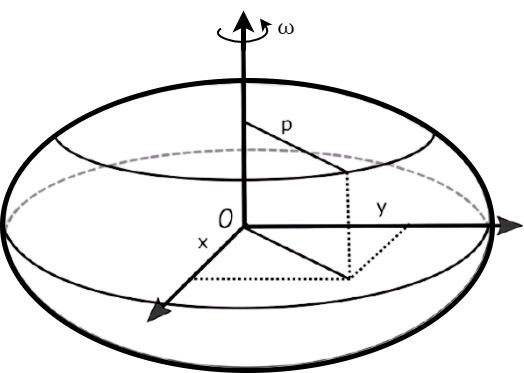
\includegraphics[scale=0.4]{figs/a.png}
	\caption{Representação esquemática da Terra considerando-a com o formato elipsoidal e com velocidade angular $\omega$. O termo $p$ representa a distância do ponto na superfície da Terra ao eixo de rotação $\mathbf{Z}$. Projetando-o no plano $\mathbf{XY}$, o ponto P pode ser definido por $(x,y,0)$.}
	\label{fig:força_centrifuga}
\end{figure} Aplicando o operador Laplaciano a $\Phi$, encontra-se:

\begin{equation} \label{eq:harmonico_phi}
\begin{gathered}
\displaystyle {\left( \frac{\partial^{2} \Phi}{\partial x^{2}}+\frac{\partial^{2} \Phi}{\partial y^{2}}+\frac{\partial^{2} \Phi}{\partial z^{2}}\right) = \nabla^{2}\Phi} \\
\displaystyle {\nabla^{2}\Phi = 2\omega^{2}}.
\end{gathered}
\end{equation}

A relação~\ref{eq:harmonico_phi} mostra que $\Phi$ não satisfaz a equação \ref{eq:laplaciano} e que, portanto, não é um potencial harmônico. É importante observar que $\Phi$ age somente sobre corpos vinculados a Terra (i.e., região compreendida dentro da distância conferida ao raio terrestre R) \cite{escobar2000}. Assim, corpos que não sofram o efeito de rotação da Terra estão sujeitos apenas a $V$ \cite{torge}. A combinação linear entre os potenciais gravitacional e centrífugo fornece o potencial de gravidade ou geopotencial ($W$) da Terra Real \cite{hofmann2005}. Logo, fica viável definir $W$ de acordo com a soma das equações \ref{eq:integral_potencial_gravitacional} e \ref{eq:integral_potencial_centrifugo}:
\begin{equation} \label{eq:integral_potencial_W}
\displaystyle{W = V + \Phi }.
\end{equation} Aplicando o operador Laplaciano sobre o potencial de gravidade $W$, verifica-se o mesmo resultado obtido na relação \ref{eq:harmonico_phi}, conferindo a esse a categoria de potencial não harmônico.

%\subparagraph{\textit{Terra Real}:} A \textit{Terra Real} foi mencionada no parágrafo anterior e será aqui conceituada. Ela corresponde ao próprio corpo sólido chamado Terra, limitada, basicamente, pela sua superfície física que divide massas litosféricas e líquidas da sua atmosfera. O assoalho oceânico representa o limite entre corpos sólidos e massas oceânicas \cite{torge2001geodesy}. Como não foi encontrada nenhuma função analítica consistente capaz de representar as complexas irregularidades da superfície da Terra Real (topografia continental e do assoalho oceânico), foi estabelecida a \textit{Terra Normal}, constituída por uma superfície fictícia que se estende por baixo dos continentes. A sua geometria é a de um elipsoide de revolução, cujo propósito é representar a Terra Real da melhor forma possível.

\subparagraph{\textit{Terra Normal}:}  Consiste em uma superfície fictícia que se estende por baixo dos continentes. A sua geometria é a de um elipsoide de revolução, cujo propósito é representar a Terra Real da melhor forma possível. A Terra Normal segue algumas condições predefinidas: possui a mesma massa da Terra Real, incluindo a massa da atmosfera; mesma velocidade angular $\omega$ da Terra Real; sua origem coincide com o centro de massa médio da Terra, e o semieixo menor b, coincide com o eixo de rotação médio da Terra. Por fim, sua superfície limitante é equipotencial do seu próprio campo de gravidade \cite{heiskanen1967, hofmann2005} e numericamente igual ao potencial $U=U_0$ \cite{escobar2000}.

O potencial de gravidade normal $U$, referente à Terra Normal é obtido por meio da combinação linear entre o seu potencial gravitacional $\tilde{V}$ e o potencial centrífugo $\Phi$

\begin{equation} \label{eq:esferopotencial}
\displaystyle {U = \tilde{V} + \Phi}.
\end{equation}
O símbolo $\mathbf{\sim}$ foi usado para distinguir este potencial gravitacional oriundo dos efeitos gravitacionais da Terra Normal daquele referente à Terra Real. É possível definir uma função para $\tilde{V} $ análoga à equação~\ref{eq:integral_potencial_gravitacional}
\begin{equation} \label{eq:integral_potencial_gravitacional_normal}
\displaystyle {\tilde{V} = G \int_{Terra\,\,Normal} \frac{\tilde{\rho}(r') dv'}{| \mathbf{r} - \mathbf{r'} |},} 
\end{equation}
em que $\tilde{\rho}(r')$ corresponde à distribuição de densidade interna da Terra Normal. Note que o potencial centrífugo é o mesmo da Terra Real por definição \cite{heiskanen1967} (vide equação~\ref{eq:integral_potencial_W}). O fato de $\Phi$ ser o mesmo em ambos os casos se dá pelo estabelecimento das condições e parâmetros impostos ao elipsoide de referência escolhido, que são equivalentes à Terra Real. Analogamente a $W$, $U$ não satisfaz a equação \ref{eq:laplaciano}, logo não é um potencial harmônico.

\subsection{Harmônicos esféricos}

O potencial de gravidade de um corpo com distribuição de massas homogênea e  geometria simples admite, em geral, uma representação matemática exata e consistente. No entanto, o potencial de um corpo com distribuição de massas heterogênea e forma geométrica complexa como a Terra só pode ser obtido através de aproximações. Em geral, estas aproximações podem ser expressas matematicamente por meio de séries descritas em coordenadas esféricas $(r,\phi,\lambda)$ (i.e., raio, colatitude e longitude, respectivamente), onde o número de termos depende da resolução dos dados, indicando o grau de aproximação \cite{modelagem_matematica2,molina}. Muitas são as alternativas para representar uma função por meio de séries de potências. Nesta seção, trataremos com maior especificidade da expansão em harmônicos esféricos.

Os harmônicos esféricos são funções harmônicas que representam a variação espacial de um conjunto ortogonal de soluções da equação \ref{eq:laplaciano}, quando considera-se que a Terra tem o formato de uma esfera de raio R. Logo, a análise em harmônicos esféricos, permite representar uma função qualquer a partir de um conjunto de coeficientes a serem determinados por meio de um método de otimização \cite{torge2001geodesy, menke2018geophysical}. Com o efeito, é possível utilizar a expansão em harmônicos esféricos para representar o potencial gravitacional em qualquer localidade da Terra \cite{blakely1996,barthelmes2009}. Assumindo a notação de \citeonline{hofmann2006}, a equação \ref{eq:harmonico_V} em coordenadas esféricas é dada por:

\begin{equation}
\label{eq:laplaciano generico harmonicos esfericos}
\begin{gathered}
\displaystyle {\nabla^{2}V(r,\phi, \lambda)=0} \\ \\
\displaystyle {\nabla^{2}V(r,\phi, \lambda)={{r^{2}\,} {\frac{\partial^{2}V}{\partial r^{2}}} + {2r\,}{\frac{\partial V}{\partial r}} + {\dfrac{\partial^{2}V}{\partial \phi^{2}} + {\cot\phi\,}{\dfrac{\partial V}{\partial \phi}} + {\dfrac{1}{\sin^{2}\phi\,}{\dfrac{\partial^{2}V}{\partial \lambda^{2}}}}}}}.
\end{gathered}
\end{equation} Utilizando o método de separação de variáveis para resolver a equação \ref{eq:laplaciano generico harmonicos esfericos}, tem-se:

\begin{equation}
\label{eq:soluçoes separaveis}
\displaystyle {V(r,\phi,\lambda) = f(r)\,Y(\phi,\lambda)},
\end{equation} sendo $f(r)$ a componente radial da equação e $Y(\phi,\lambda)$, a componente angular. Substituindo a equação \ref{eq:soluçoes separaveis} na equação \ref{eq:laplaciano generico harmonicos esfericos}, dividindo por $f\,Y$ e rearranjando os termos de forma que apenas a função radial fique no lado esquerdo e a função angular no lado direito da igualdade, tem-se:

\begin{equation}
\label{eq:soluçoes separaveis 2}
\displaystyle{ {\frac{1}{f}\,}\left({r^{2}f''\,} + {\,\,{2r}f'}\right) = -{\frac{1}{Y}\,}\left({\frac{\partial^{2}Y}{\partial \phi^{2}}}\,\, + \,\, {\cot \phi\,}{\frac{\partial Y}{\partial \phi}}\,\, + {\frac{1}{\sin^{2}\phi \,}}{\frac{\partial^{2}Y}{\partial \lambda^{2}}}\right) }.
\end{equation} Como o lado esquerdo da igualdade depende apenas de $r$ e o lado direito de $\phi$ e $\lambda$, ambos devem ser iguais a uma constante. Portanto, podemos resolver componente radial $f(r)$ da seguinte forma:
\begin{equation}
\label{eq:sp3.a}
\displaystyle{{\frac{1}{f}\,}\left({r^{2}f''\,} + {\,\,{2r}f'}\right) =  n(n+1)},
\end{equation} onde denotamos a constante por $n(n+1)$. As possíveis soluções para a equação \ref{eq:sp3.a} são $r^{n}$ e $r^{-(n+1)}$, onde a primeira está associada a regiões internas à Terra e a segunda, exteriores à ela. Dessa forma, V pode ser representado por:

\begin{equation}
V = \begin{cases}
\label{eq:sph}
\displaystyle{\,r^{n}\,\,Y_{n}(\phi,\lambda) \rightarrow{r <R}}\\ \\
\displaystyle{\,\frac{Y_{n}(\phi,\lambda)}{r^{n+1}} \rightarrow{r > R}}
\end{cases},
\end{equation} sendo R o raio equatorial de referência da Terra. As soluções de $V$, representadas pelas equações \ref{eq:sph}, são denominadas harmônicos esféricos sólidos. Já a parte angular $Y_{n}$ é chamada de harmônicos esféricos de superfície. Retomando a equação \ref{eq:soluçoes separaveis 2} e igualando o seu lado direito, ou seja, a componente angular à constante supracitada, tem-se:

\begin{equation}
\label{eq:sp3.b}
\displaystyle{ -{\frac{1}{Y}\,}\left({\frac{\partial^{2}Y}{\partial \phi^{2}}}\,\, + \,\, {\cot \phi\,}{\frac{\partial Y}{\partial \phi}}\,\, + {\frac{1}{\sin^{2}\phi \,}}{\frac{\partial^{2}Y}{\partial \lambda^{2}}}\right) = n(n+1)}.
\end{equation} Aplicando novamente a separação de variáveis, desmembramos $Y_{n}(\phi,\lambda) = g(\phi)\,h(\lambda)$ e substituímos na equação \ref{eq:sp3.b}, obtém-se:

\begin{equation}
\label{eq:harmonicos_sep}
{\frac{\sin \phi}{g(\phi)}\,\left[ {\sin\phi \,g''(\phi)} + {\cos\phi\,g'(\phi)} + {n(n+1)\sin\phi\,g(\phi)}\right] = - \frac{h''(\lambda)}{h(\lambda)} = m^{2}},
\end{equation} em que o termo à esquerda da igualdade é uma função dependente apenas de $\phi$ e à direita, de $\lambda$. Ambos devem ser iguais a uma constante, no caso  $m^{2}$.
A partir de algumas manipulações matemáticas e considerações, que podem ser vistas em maiores detalhes em \citeonline{heiskanen1967}, é possível representar o potencial gravitacional em harmônicos esféricos:

\begin{equation}
\label{eq:V_harmonicos_esfericos}
\displaystyle {V(r,\phi, \lambda)  =\frac{GM}{r} \sum_{n=0}^{n_{max}} \sum_{m=0}^{n} \left( \frac{R}{r}\right)^{n} P_{nm}(\cos\phi)(C_{nm}^{W} \cos m\lambda + S_{nm}^{W} \sin m\lambda)},
\end{equation} em que $GM$ é o produto da constante gravitacional e da massa da Terra; $P_{nm}$ são as funções de \textit{Lengendre} totalmente normalizadas; ($C_{nm}^{W}, S_{nm}^{W}$) os coeficientes normalizados; ($n,m$) são grau e ordem dos harmônicos esféricos \cite{jekeli2000,barthelmes2009}. As soluções periódicas para cada coordenada depende dos dois inteiros ($n,m$) e é dada em termos de funções trigonométricas e dos polinômios associados de \textit{Legendre}. De acordo com a equação \ref{eq:V_harmonicos_esfericos}, os coeficientes $C_{nm}$ e $S_{nm}$ devem expressar o mais fielmente possível a distribuição de massas da Terra, para que o modelo do potencial seja representado adequadamente. A determinação de tais coeficientes é obtida por meio da resolução de hiper-sistemas lineares envolvendo os dados de satélites artificiais. Para mais detalhes acerca do tema, o leitor é convidado à \cite{heiskanen1967, torge2001geodesy,hofmann2006}.

\subsection{Gravidade}

O vetor gravidade $\mathbf{g}$, produzido pela Terra Real em um determinado ponto, pode ser definido como o \textit{gradiente} do potencial de gravidade exercida por unidade de massa \cite{hofmann2005}.

\begin{equation} \label{eq:vetor_gravidade_g}
\displaystyle {\mathbf{g}=  \mathbf{\nabla} {W}} .
\end{equation} A gravidade é uma grandeza vetorial que pode ser interpretada como um tipo de aceleração devido às interações entre massas. Logo, o vetor gravidade contém a aceleração da gravidade  em $Gal$, em homenagem a \textit{Galileu Galilei} onde $1 gal= 1 cm.s^{-2}$ \cite{hofmann2005,escobar2000}. Na superfície terrestre, nota-se uma variação na magnitude da gravidade de cerca de $5$ Gal, sendo maior nos polos e menor na região equatorial. Essa variação é resultado da componente centrífuga da gravidade \cite{escobar2000,geodesia}. 

Substituindo a equação~\ref{eq:integral_potencial_W} na \ref{eq:vetor_gravidade_g}, nota-se que o vetor gravidade $\mathbf{g}$ pode ser expresso pela combinação linear de $\mathbf{a}_V$ e $\mathbf{a}_C$, da seguinte maneira:

\begin{equation} \label{eq:vec_g_comb_linear}
\displaystyle {\mathbf{g} = \underbrace{\mathbf{\nabla} { V }}_{\mathbf{a}_V} + \underbrace{\mathbf{\nabla} {\Phi} }_{\mathbf{a}_C} },
\end{equation} em que $\mathbf{a}_V$ é denominado aceleração gravitacional ou atração gravitacional \cite{hofmann2005} e $\mathbf{a}_C$ a aceleração centrífuga, que, assim como $\mathbf{g}$, são medidas em unidades de $ms^{-2}$ no SI \cite{torge}. A Figura \ref{fig:aceleracoes} mostra uma representação esquemática da eq. \ref{eq:vec_g_comb_linear} em que as setas azuis representam $\mathbf{a}_V$, as verdes, $\mathbf{a}_C$ e as vermelhas a soma vetorial das duas anteriores, $\mathbf{g}$.

\begin{figure}[!h]
	\centering
	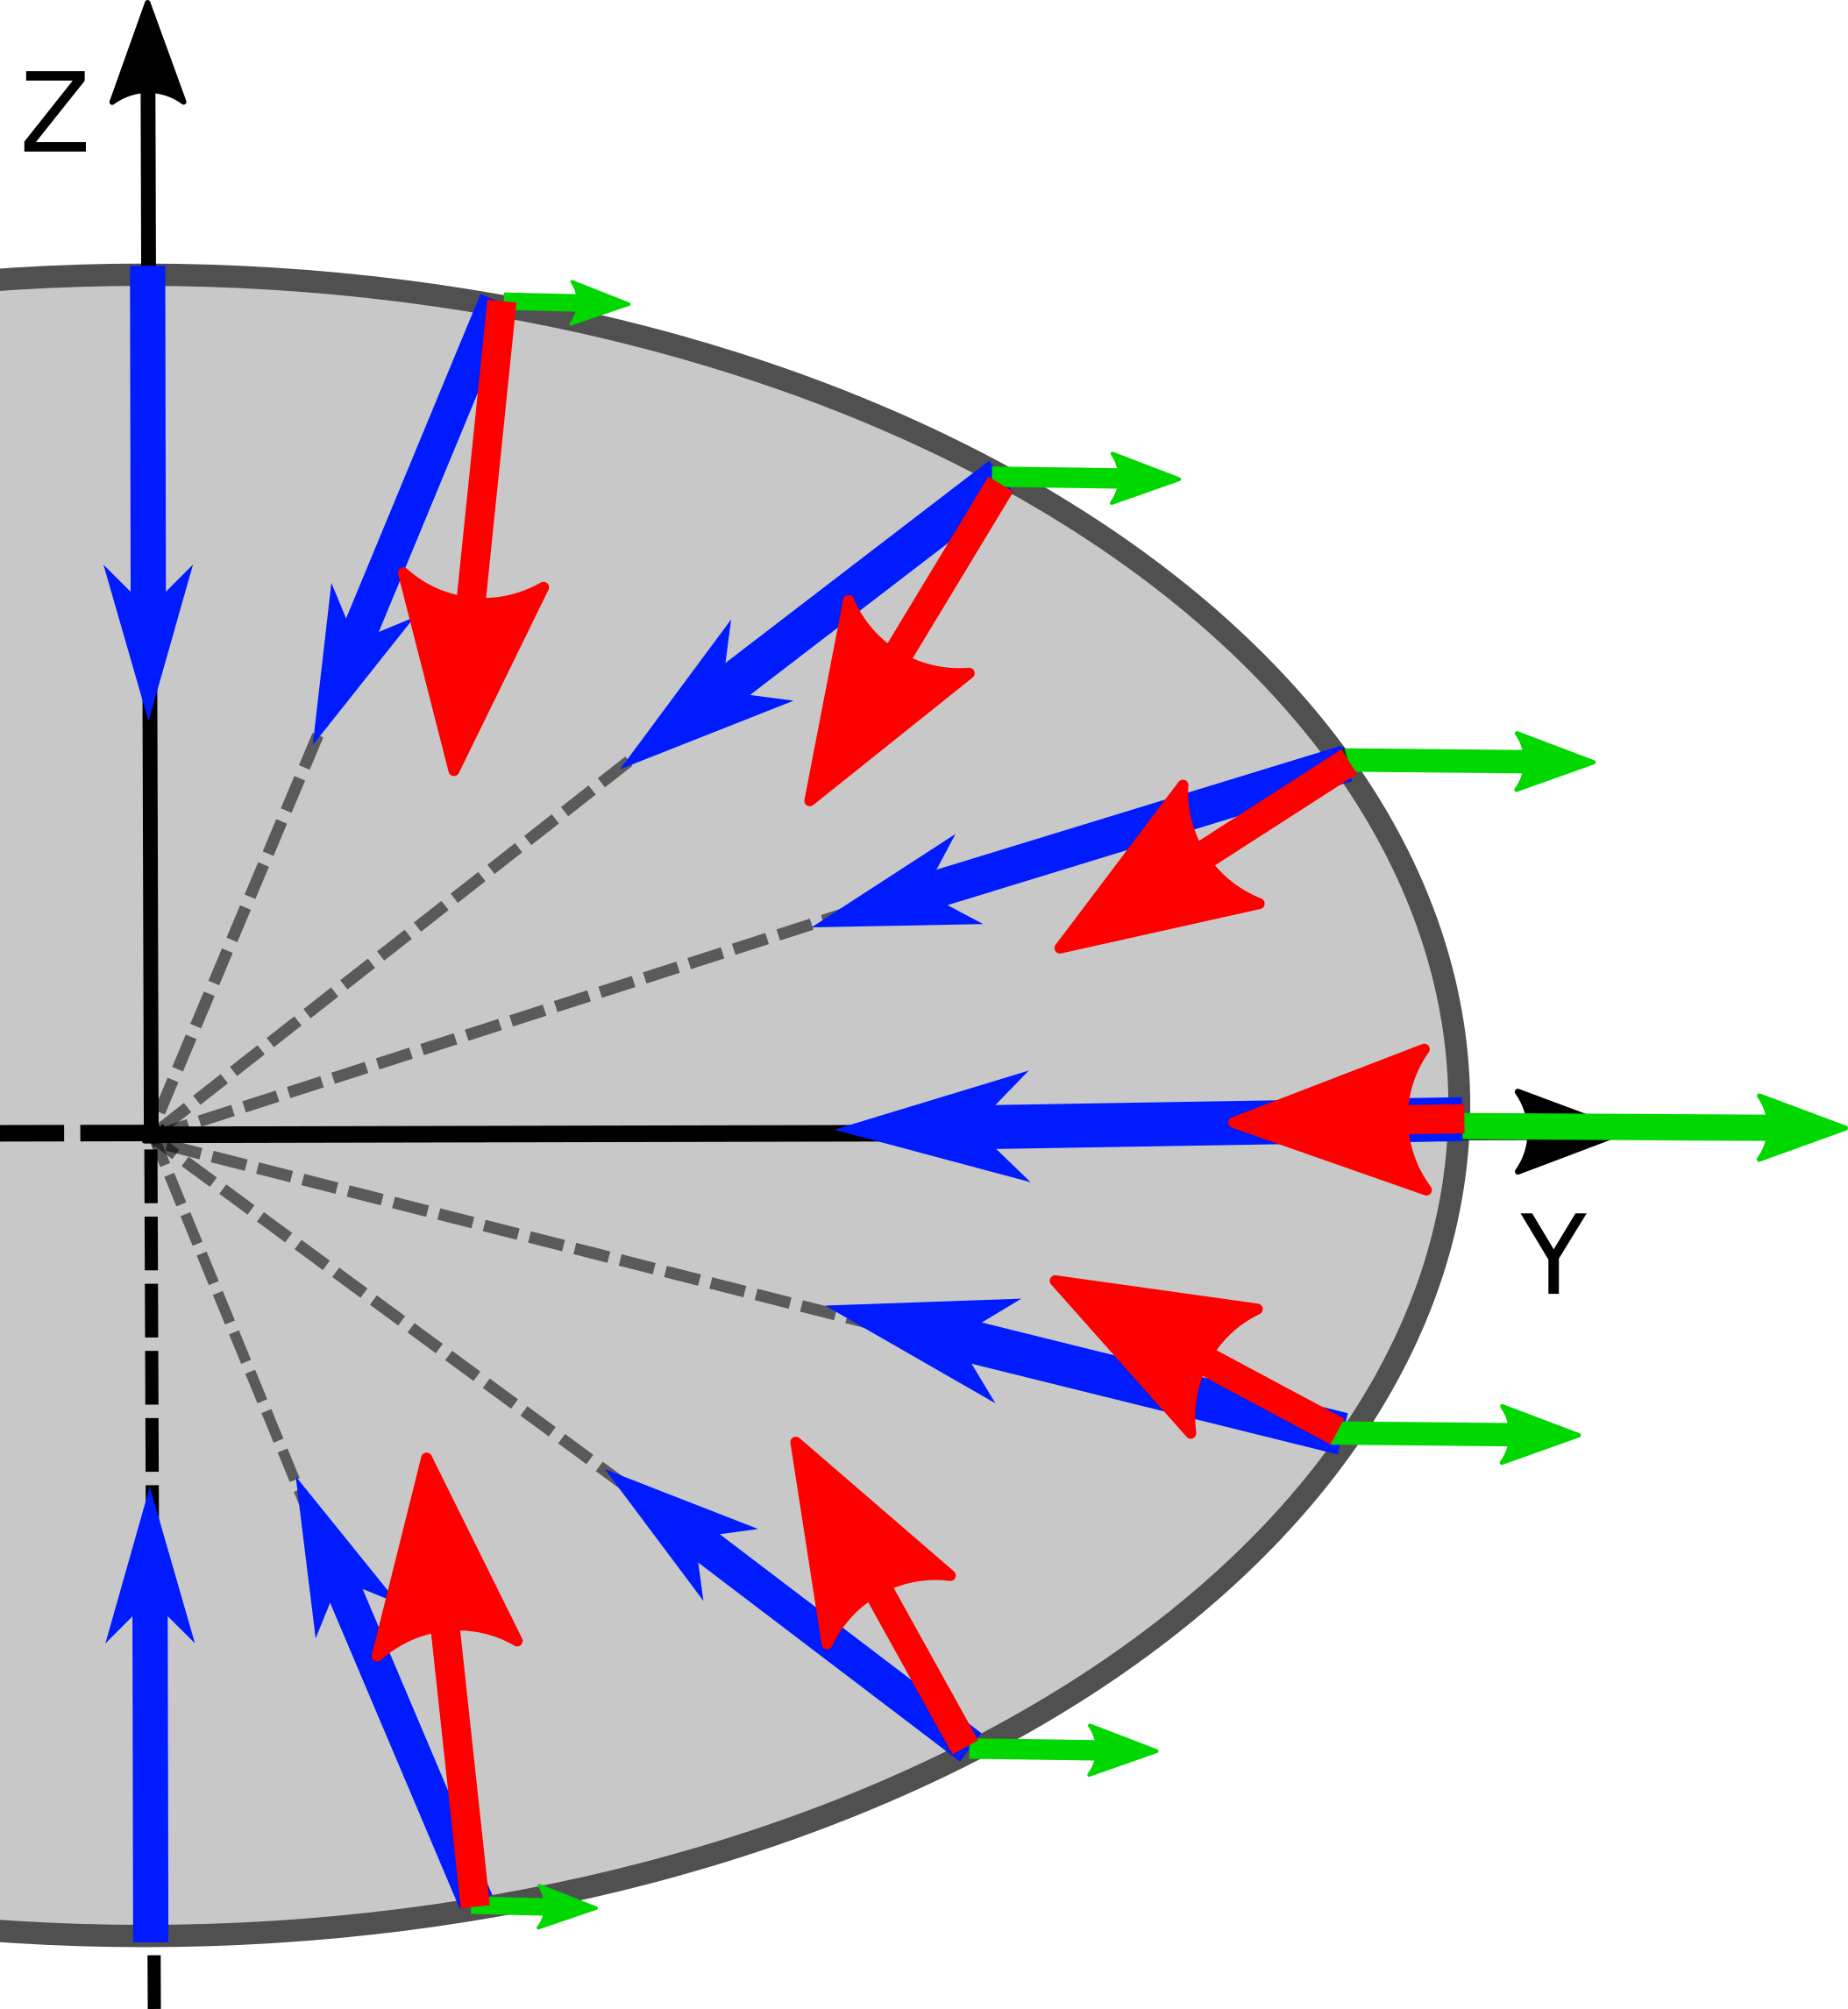
\includegraphics[scale=0.3]{figs/vec.png}
	\caption{Representação esquemática da visão lateral da Terra elipsoidal. Percorrendo dos polos ao equador, há uma considerável diminuição de $\mathbf{g}$ (setas vermelhas) devido à maior atuação de $\mathbf{a}_C$ (setas verdes). $\mathbf{a}_V$ é representado pelas setas azuis}
	\label{fig:aceleracoes}
\end{figure}

A gravidade, por sua vez, é definida como o módulo do vetor gravidade
\begin{equation} \label{eq:gravidade_g}
\displaystyle {g = \parallel \mathbf{g} \parallel }.
\end{equation}

Analogamente, é possível obter relações semelhantes para a Terra Normal. Neste caso, o vetor gravidade normal $(\boldsymbol{\gamma})$ para a Terra Normal é definido como o gradiente do potencial de gravidade normal $U$:

\begin{equation} \label{eq:vec_gravidade_normal}
\displaystyle {\boldsymbol{\gamma} = \mathbf{\nabla} U  },
\end{equation} e sua intensidade, conhecida por gravidade normal, é:

\begin{equation} \label{eq:gravidade_normal}
\displaystyle {\gamma = \parallel \boldsymbol{\gamma} \parallel }.
\end{equation}

\subsection{Equipotenciais}

Segundo \citeonline{blakely1996}, as superfícies equipotenciais (ou superfícies de nível), apresentam potencial constante ao longo de toda superfície. No caso particular de $W$, as superfícies equipotenciais são denominadas de \textit{geopes} \cite{arana2009}. O \textit{geope} fundamental é o geoide ($W = W_{0}$), cuja superfície equipotencial do campo de gravidade da Terra Real coincide com o nível médio não perturbado dos mares. O geoide possui formato ondulatório levemente irregular, idealizado com base em estudos gravimétricos, que acompanha as variações da estrutura de distribuição de massas da Terra Real \cite{matos2016}. Se for tomado como referência o campo de gravidade normal, sua equipotencial será uma superfície regular, denominada \textit{esferope}. O \textit{esferope} fundamental é representado pela própria superfície do elipsoide, em que ($U=U_0$); ela deve ser estabelecida de tal forma que se aproxime do geoide \cite{barthelmes2009}. 

As linhas do campo de gravidade em qualquer ponto são sempre perpendiculares às superfícies equipotenciais e descrevem a direção do vetor gravidade. Portanto, nenhum trabalho é realizado na movimentação de uma partícula ao longo de uma superfície equipotencial \cite{torge}, já que o vetor gravidade é sempre perpendicular à superfície, o que equivale dizer que o produto escalar é nulo. Além de serem constantes e nunca se cruzarem, a distância entre as superfícies é inversamente proporcional ao campo de gravidade. Logo, a distância entre elas reflete a densidade das linhas de campo, ou seja, um campo terá maior intensidade em regiões onde superfícies equipotenciais adjacentes estão mais próximas \cite{blakely1996}.

As superfícies do geoide e do elipsoide podem servir de superfícies de referência para o posicionamento de pontos no espaço. Por exemplo: seja um ponto $P$ sobre a superfície física da Terra ($SFT$). Se a superfície de referência for o geoide, este ponto estará a uma distância $H$ em relação a ele. Esta distância pode ser entendida como uma altitude e, por estar associada ao geoide, é nomeada altitude ortométrica. Por outro lado, se o referencial for a superfície do elipsoide, este mesmo ponto terá a altitude geométrica ($h$). A diferença entre as duas superfícies fornece a ondulação geoidal ($N$): 

\begin{equation}
\label{eq:geometric}
\displaystyle {h\approx H+N}.
\end{equation}

\begin{figure}[H]
	\centering
	\includegraphics[scale=0.17]{figs/N.png}
	\caption{Ondulação geoidal da Terra. Retirado do \textit{International Centre for Global Earth Models} \href{http://icgem.gfz-potsdam.de/home}{(ICGEM)}.}
	\label{fig:N}
\end{figure}
\FloatBarrier
A ondulação geoidal da Figura \ref{fig:N} representa a distância entre as superfícies do geoide e do elipsoide ao redor do globo, que fica em torno $\pm 100m$ \cite{jekeli2000}. As ondulações do geoide se distribuem pela Terra e podem ser calculadas de acordo com um modelo de ondulação geoidal. Para exemplificar, foi calculado o valor de $N$ para um ponto de observação localizado na portaria do edifício do \textit{Instituto de Geociências da Universidade Federal Fluminense} ($22.90$º$S$, $43.13$º$W$), a partir do \textit{Modelo de Ondulação Geoidal do Brasil} (MAPGEO2015) do \textit{Instituto Brasileiro de Geografia e Estatística} (IBGE). Este é o modelo de ondulação geoidal brasileiro mais recente, e permite calcular $N$ em um ponto ou conjunto de pontos do território brasileiro a partir das suas coordenadas planimétricas. Para mais detalhes acerca da metodologia utilizada neste modelo, o leitor é convidado a \citeonline{mapgeo2015}. Para o ponto em questão, obteve-se uma ondulação de $-6.00$ m. Ou seja, significa que nesta localidade o geoide esta cerca de $6$ m abaixo do elipsoide. A Figura \ref{fig:superficies equipotenciais} esquematiza as principais superfícies e suas respectivas altitudes.

\begin{figure}[H]
	\centering
	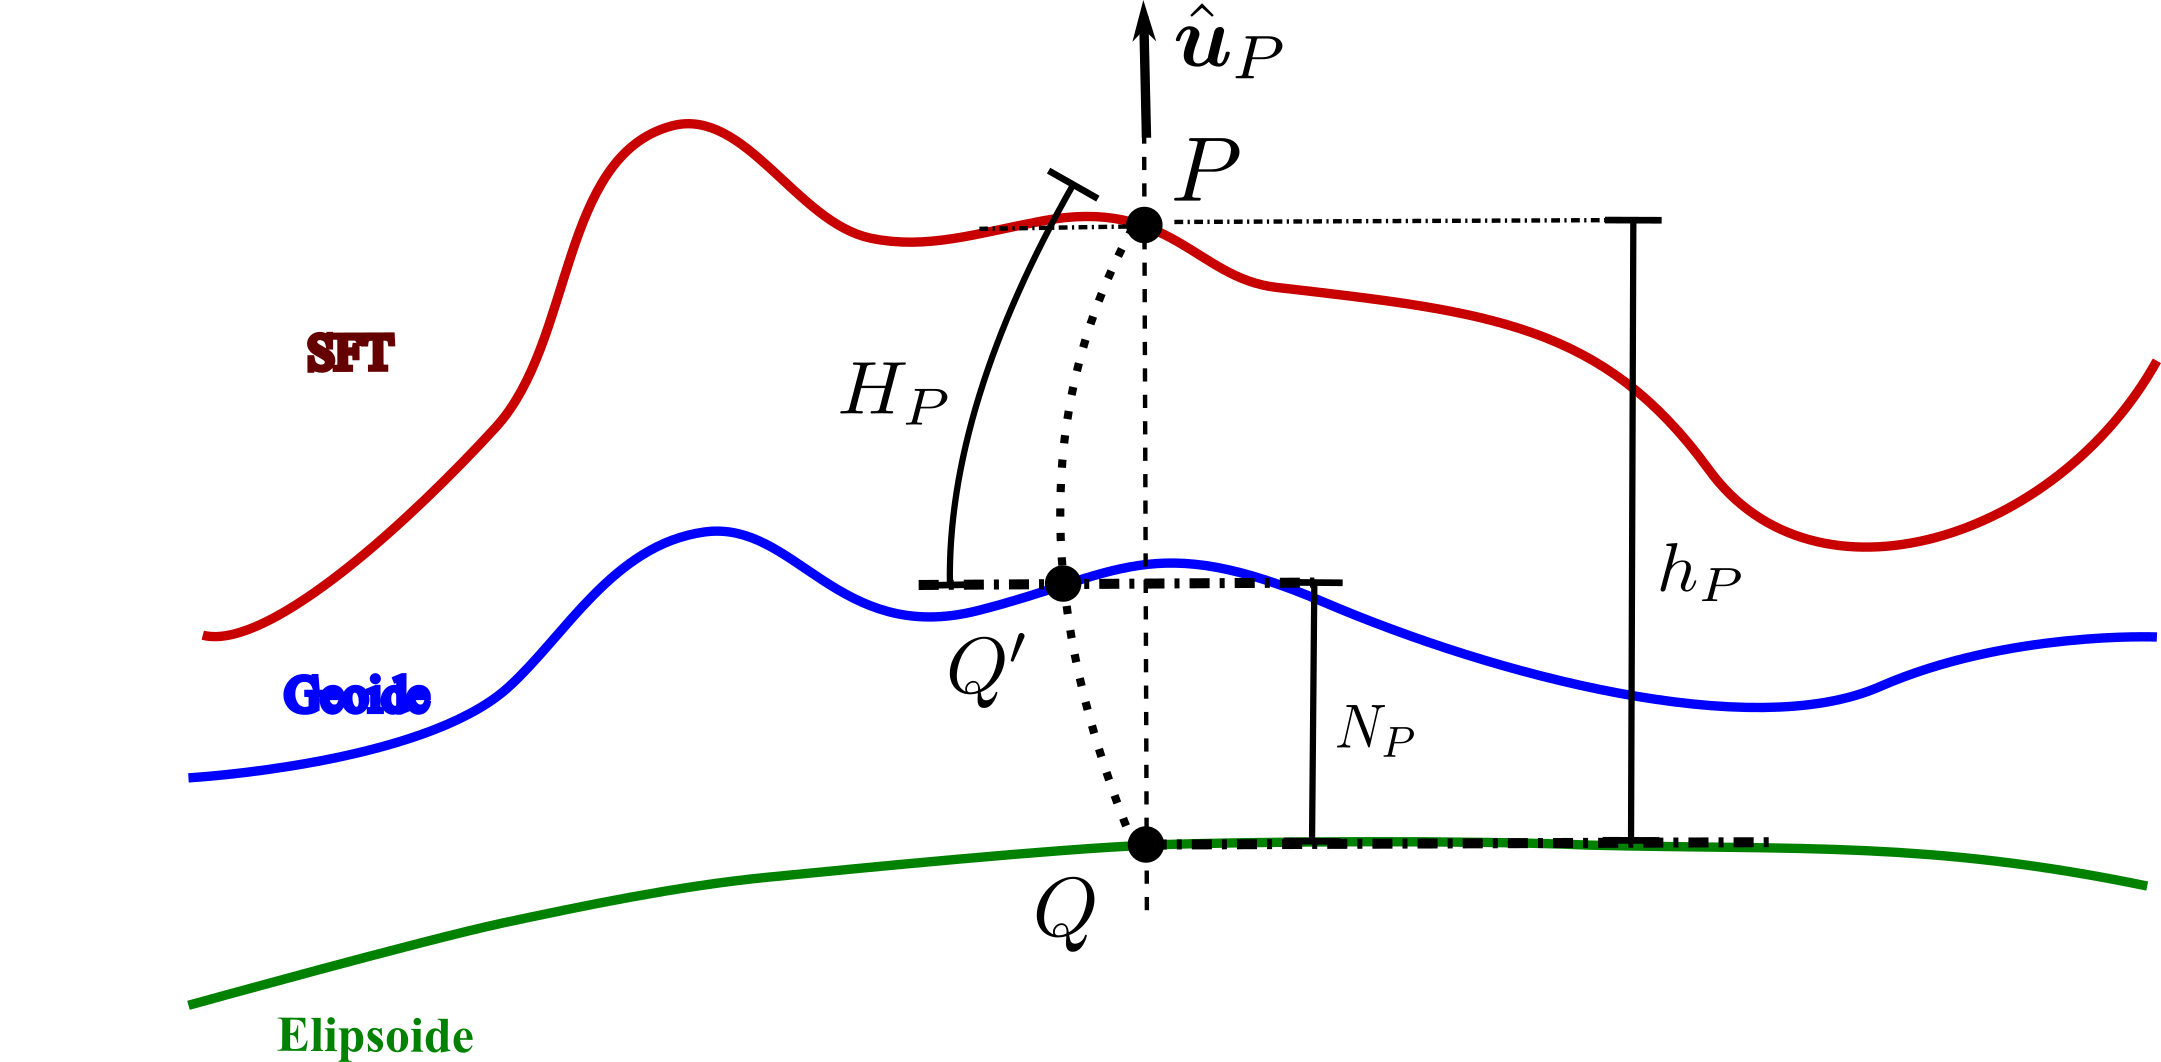
\includegraphics[scale=1.2]{figs/s.png}
	\caption{Modelo esquemático das superfícies equipotenciais, altitudes geométrica ($h$) e ortométrica ($H$) e ondulação geoidal ($N$).}
	\label{fig:superficies equipotenciais}
\end{figure}

\subsection{Anomalia e distúrbio de gravidade}

Considere um ponto $P$ sobre a $SFT$. Projetando-o sobre o geoide e o elipsoide, acompanhando a linha de prumo, são fixados os pontos $Q^{\prime}$ e $Q$, respectivamente, conforme a Figura \ref{fig:disturbio}. O vetor anomalia de gravidade ($\Delta \mathbf{g}_P$) é uma grandeza muito utilizada na geofísica e pode ser definida como sendo a diferença entre $\mathbf{g}_{Q^{\prime}}$ e $\mathbf{\gamma}_{Q}$, ou seja, a diferença entre o vetor gravidade avaliado sobre o geoide (Q') e o vetor gravidade normal no elipsoide (Q).

\begin{equation}
\label{eq:vetor_anomalia de gravidade}
\displaystyle {\Delta \mathbf{g}_P = \mathbf{g}_{Q^{\prime}} - \boldsymbol{\gamma}_Q}.
\end{equation} O vetor distúrbio de gravidade ($\mathbf{\delta g}_P$) por outro lado, mais conhecido na geodésia, é dado por \cite{torge,hofmann2006}:

\begin{equation}
\label{eq:vetor_disturbio}
\displaystyle {\delta \mathbf{g}_P = \mathbf{g}_P - \boldsymbol{\gamma}_P},
\end{equation} e o distúrbio de gravidade é calculado fazendo a diferença entre as equações \ref{eq:gravidade_g} e \ref{eq:gravidade_normal}, de forma que:

\begin{equation}
\label{eq:disturbio}
\displaystyle {\delta g_P = \parallel\mathbf{g}_P\parallel - \parallel\boldsymbol{\gamma}_P\parallel}.
\end{equation}

\begin{figure}[H]
	\centering
	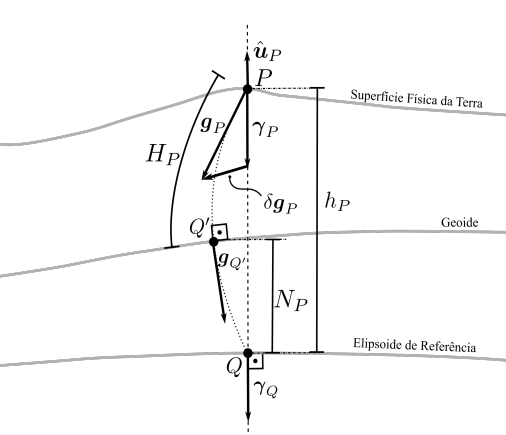
\includegraphics[scale=0.5]{figs/disturbio_de_gravidade.png}
	\caption{Representação esquemática dos vetores de gravidade em um ponto $P$ sobre a superfície física da Terra.	$\mathbf{g}_P$ é o vetor gravidade, $\gamma_{P}$ é o vetor de gravidade normal, $\delta g_{P}$ é o vetor de distúrbio de gravidade, $\mathbf{\hat{u}}_{P}$ é vetor unitário da equação \ref{eq:vetores_unitarios}, $g_{Q}$ é o vetor de gravidade em um ponto ${Q'}$ sobre o geoide, $\gamma_{Q}$ é o vetor de gravidade normal em um ponto ${Q}$ sobre o elipsoide, $h_{P}$ é a altitude geométrica, $H_{P}$ é a altitude ortométrica e $N_{P}$ é a ondulação geoidal associadas ao ponto ${P}$. Os pontos ${P}$ e ${Q}$ possuem as mesmas latitude e longitude. A linha pontilhada $\overline{PQ}$ é \textit{normal} ao elipsoide de referência e representa a linha de campo associada ao campo de gravidade normal. Retirado de \citeonline{kristoffer}}.
	\label{fig:disturbio}
\end{figure}

 

A diferença entre o potencial de gravidade da Terra Real ($W$) e o potencial de gravidade da Terra Normal ($U$), no mesmo ponto $P$, fornece o potencial anômalo ou perturbador $T$ \cite{escobar2000,hofmann2006} 

\begin{equation} \label{eq:potencial_anomalo}
\begin{gathered}
\displaystyle {T_{P} = W_{P} - U_{P}} \\
\displaystyle {T_{P} = V_{P} - \tilde{V_{P}} }.
\end{gathered}
\end{equation} Substituindo as equações~\ref{eq:integral_potencial_gravitacional} e \ref{eq:integral_potencial_gravitacional_normal} em \ref{eq:potencial_anomalo}, verifica-se que $T$ é produzido pela distribuição de massas anômalas $(\Delta \rho)$,

\begin{equation} \label{eq:massas_anomalas}
\displaystyle { T = G \int_{v_0} \frac{\Delta \rho dv'}{| \mathbf{r} - \mathbf{r'} |} }
\end{equation} em que $v_{0}$ é a diferença entre Terra Real e Terra normal, $\Delta \rho = \rho - \tilde{\rho}$. Por se tratar do mesmo ponto, $T$ independe de $\Phi$ e seu efeito é puramente gravitacional, satisfazendo a equação \ref{eq:laplaciano}, ou seja, $T$ é um potencial harmônico \cite{lopes2006}.

Levando em conta as relações~\ref{eq:vetor_gravidade_g} e \ref{eq:vec_gravidade_normal}, conclui-se que $\delta \mathbf{g}_P$ é o \textit{gradiente} do potencial perturbador $T$  \cite{heiskanen1967,hofmann2006}:

\begin{equation} \label{eq:disturbio de gravidade=potencial anomalo}
\begin{gathered}
\displaystyle {\mathbf{\delta g}_{P} = \mathbf{\nabla} W_{P}-\mathbf{\nabla} U_{P}} \\
\displaystyle {\mathbf{\delta g}_{P} = \mathbf{\nabla} T_{P}}.
\end{gathered}
\end{equation} 

É imprescindível enfatizar que a anomalia de gravidade no ponto $P$ sobre a $SFT$ é calculada usando a gravidade sobre o geoide e a gravidade normal sobre o elipsoide. Desta forma, a remoção da parte centrífuga do dado não é realizada em sua totalidade. A anomalia de gravidade continua apresentando o resultado da combinação linear de efeitos gravitacionais e centrífugos, mesmo que em menor escala. Ela é amplamente utilizada como dado de entrada em vários estudos na literatura e é comumente associada ao potencial perturbador por meio da aproximação conhecida pela equação fundamental da geodésia \cite{arana2009}. Sob o aspecto da teoria do potencial e segundo os argumentos apresentados, o distúrbio de gravidade é a grandeza mais acurada para ser aplicada pois avalia $g$ e $\gamma$ no mesmo ponto P conforme mostrado na Figura \ref{fig:disturbio}. Para efeito de comparação, as Figuras \ref{subfig:anomalia}.a e b exemplificam a anomalia e distúrbio de gravidade, respectivamente, sobre a América do Sul. A Figura \ref{subfig:anomalia}.c apresenta o mapa de diferença entre distúrbio e anomalia de gravidade. Pode-se constatar que as principais diferenças se encontram na região dos Andes (valores positivos) e na porção Norte da América do Sul (valores negativos). Adicionalmente, pode-se verificar algumas disformidades de valores negativos na porção continental brasileira. Além disso, nota-se similaridades das componentes de longo comprimento de onda entre o mapa de diferenças e o da ondulação, conforme apresentado na Figura \ref{subfig:anomalia}.d.

\begin{figure}[H]
	\centering
	\subfloat[]{\includegraphics[scale=0.36]{figs/anom_AS.png}}
	\qquad
	\subfloat[]{\includegraphics[scale=0.36]{figs/delta_AS.png}}
	\qquad
	\subfloat[]{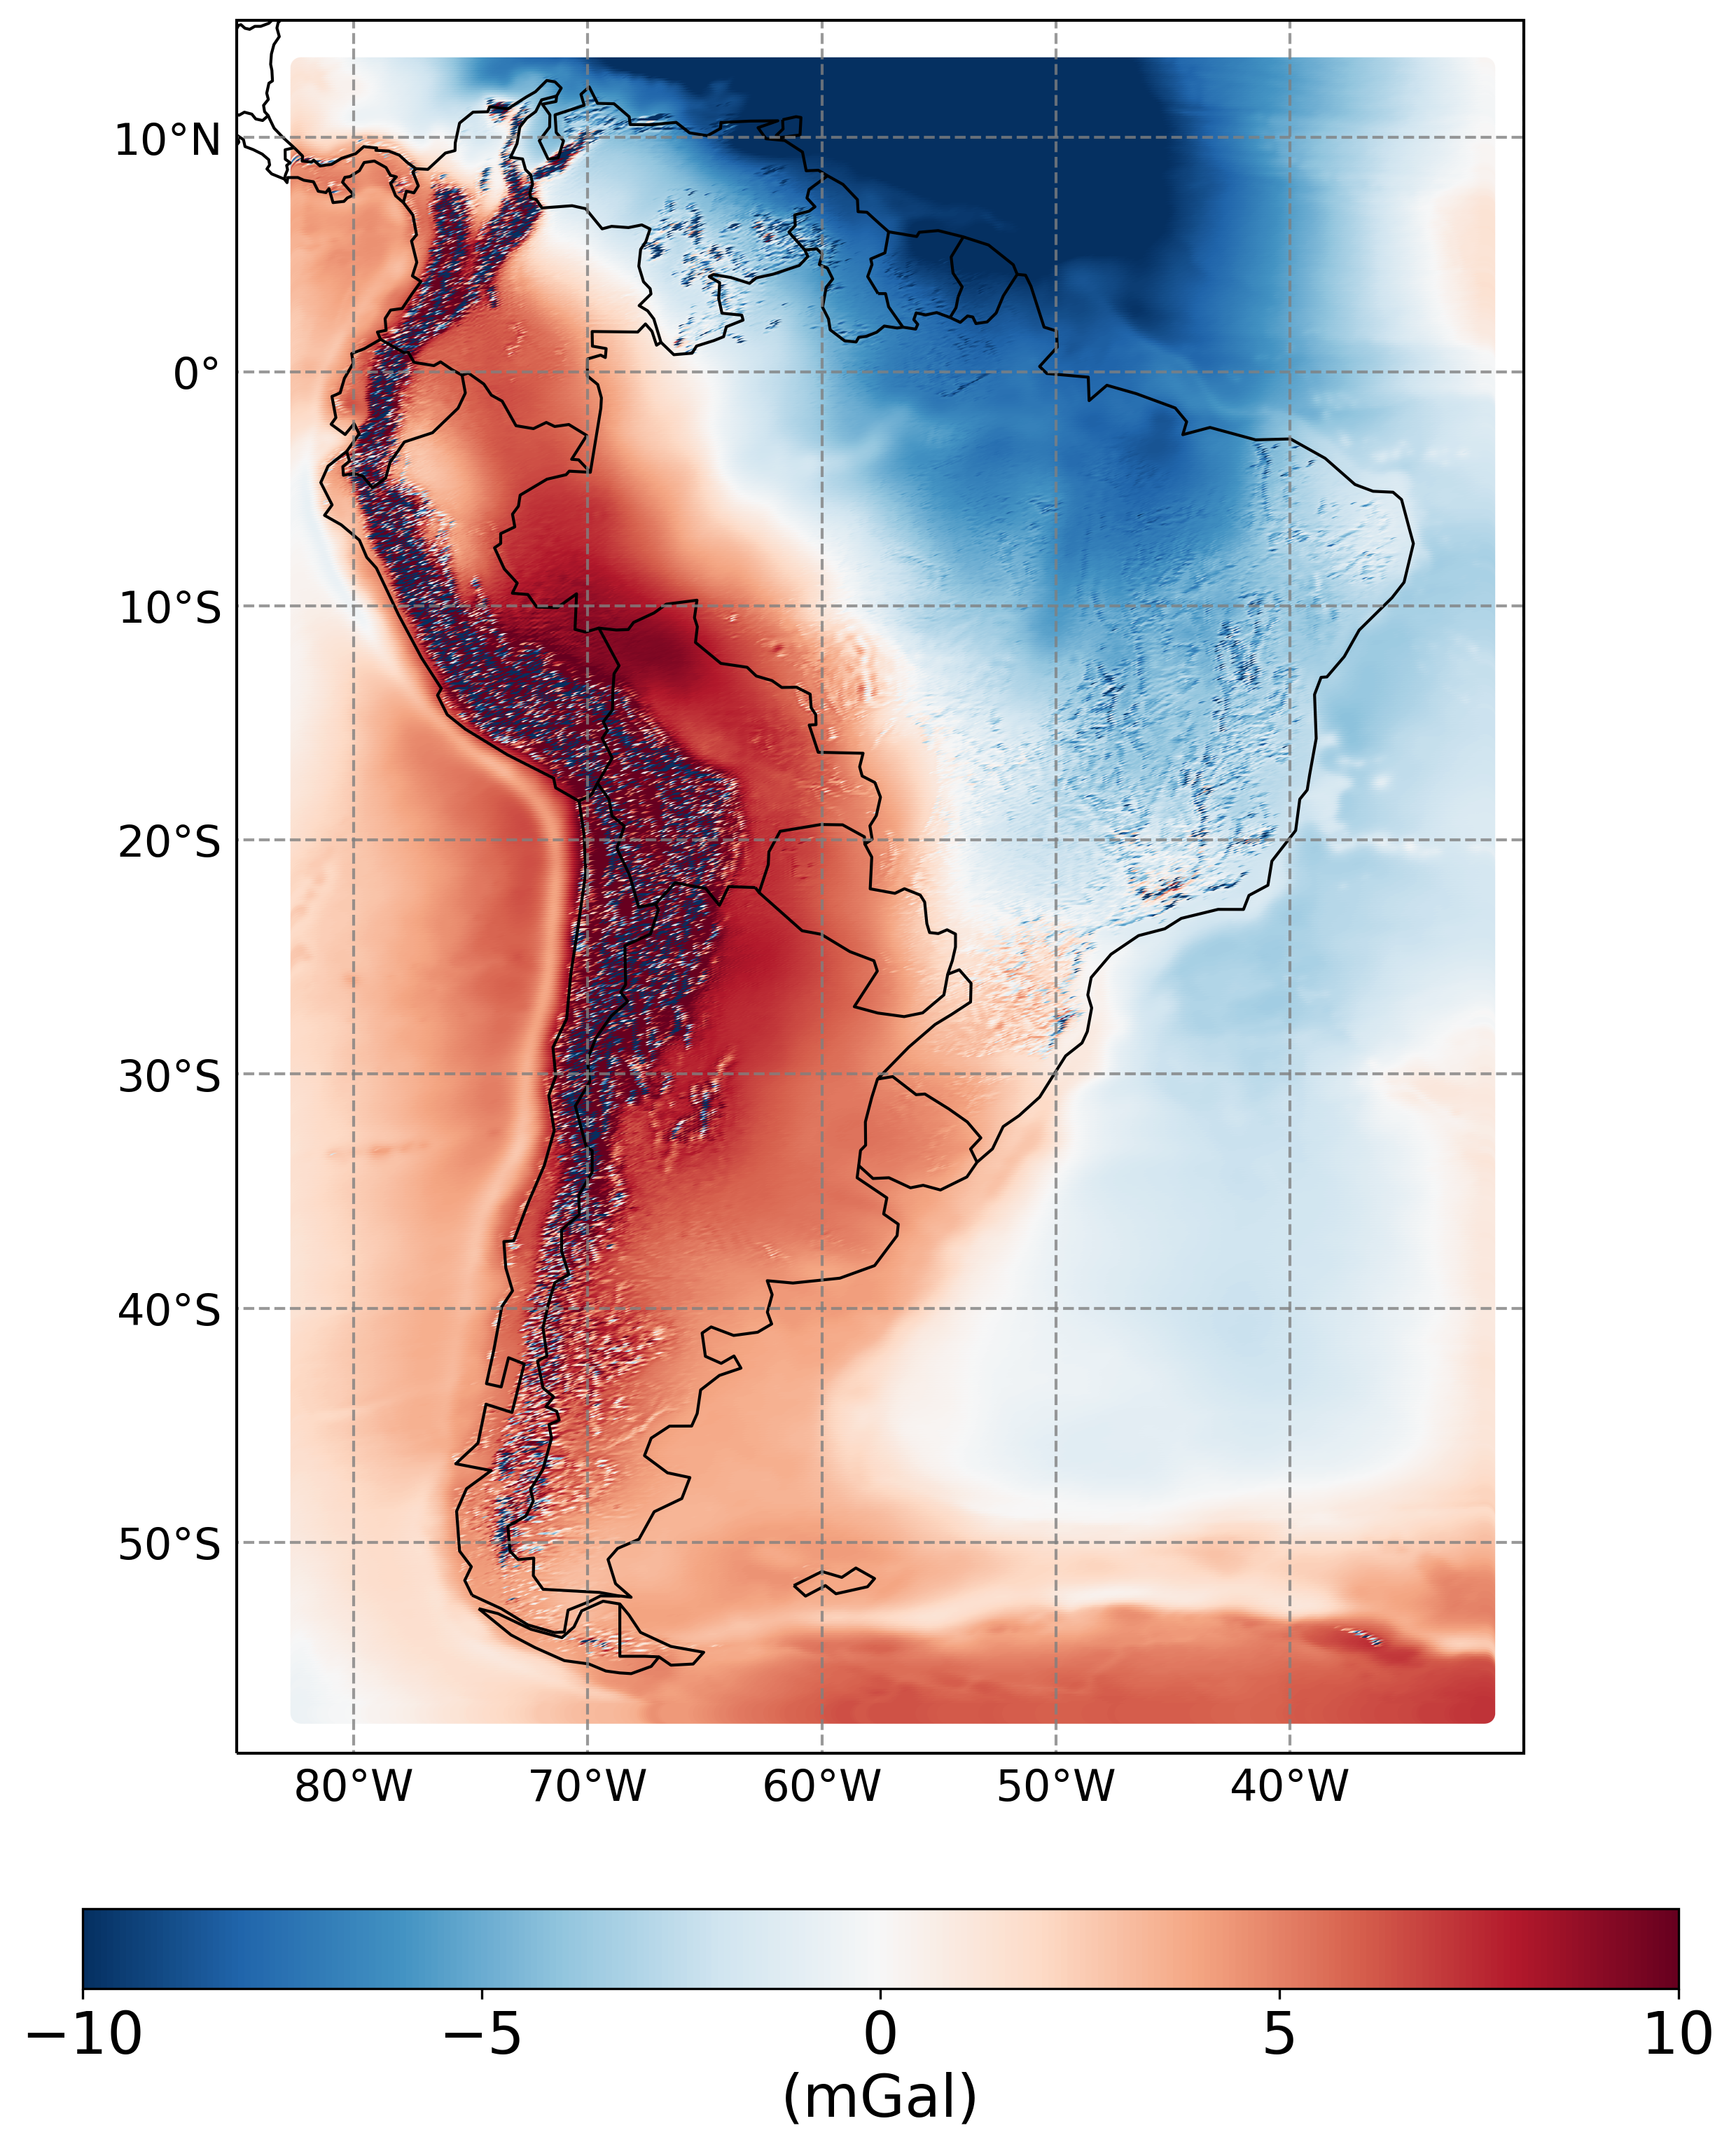
\includegraphics[scale=0.36]{figs/R_AS.png}}
	\qquad
	\subfloat[]{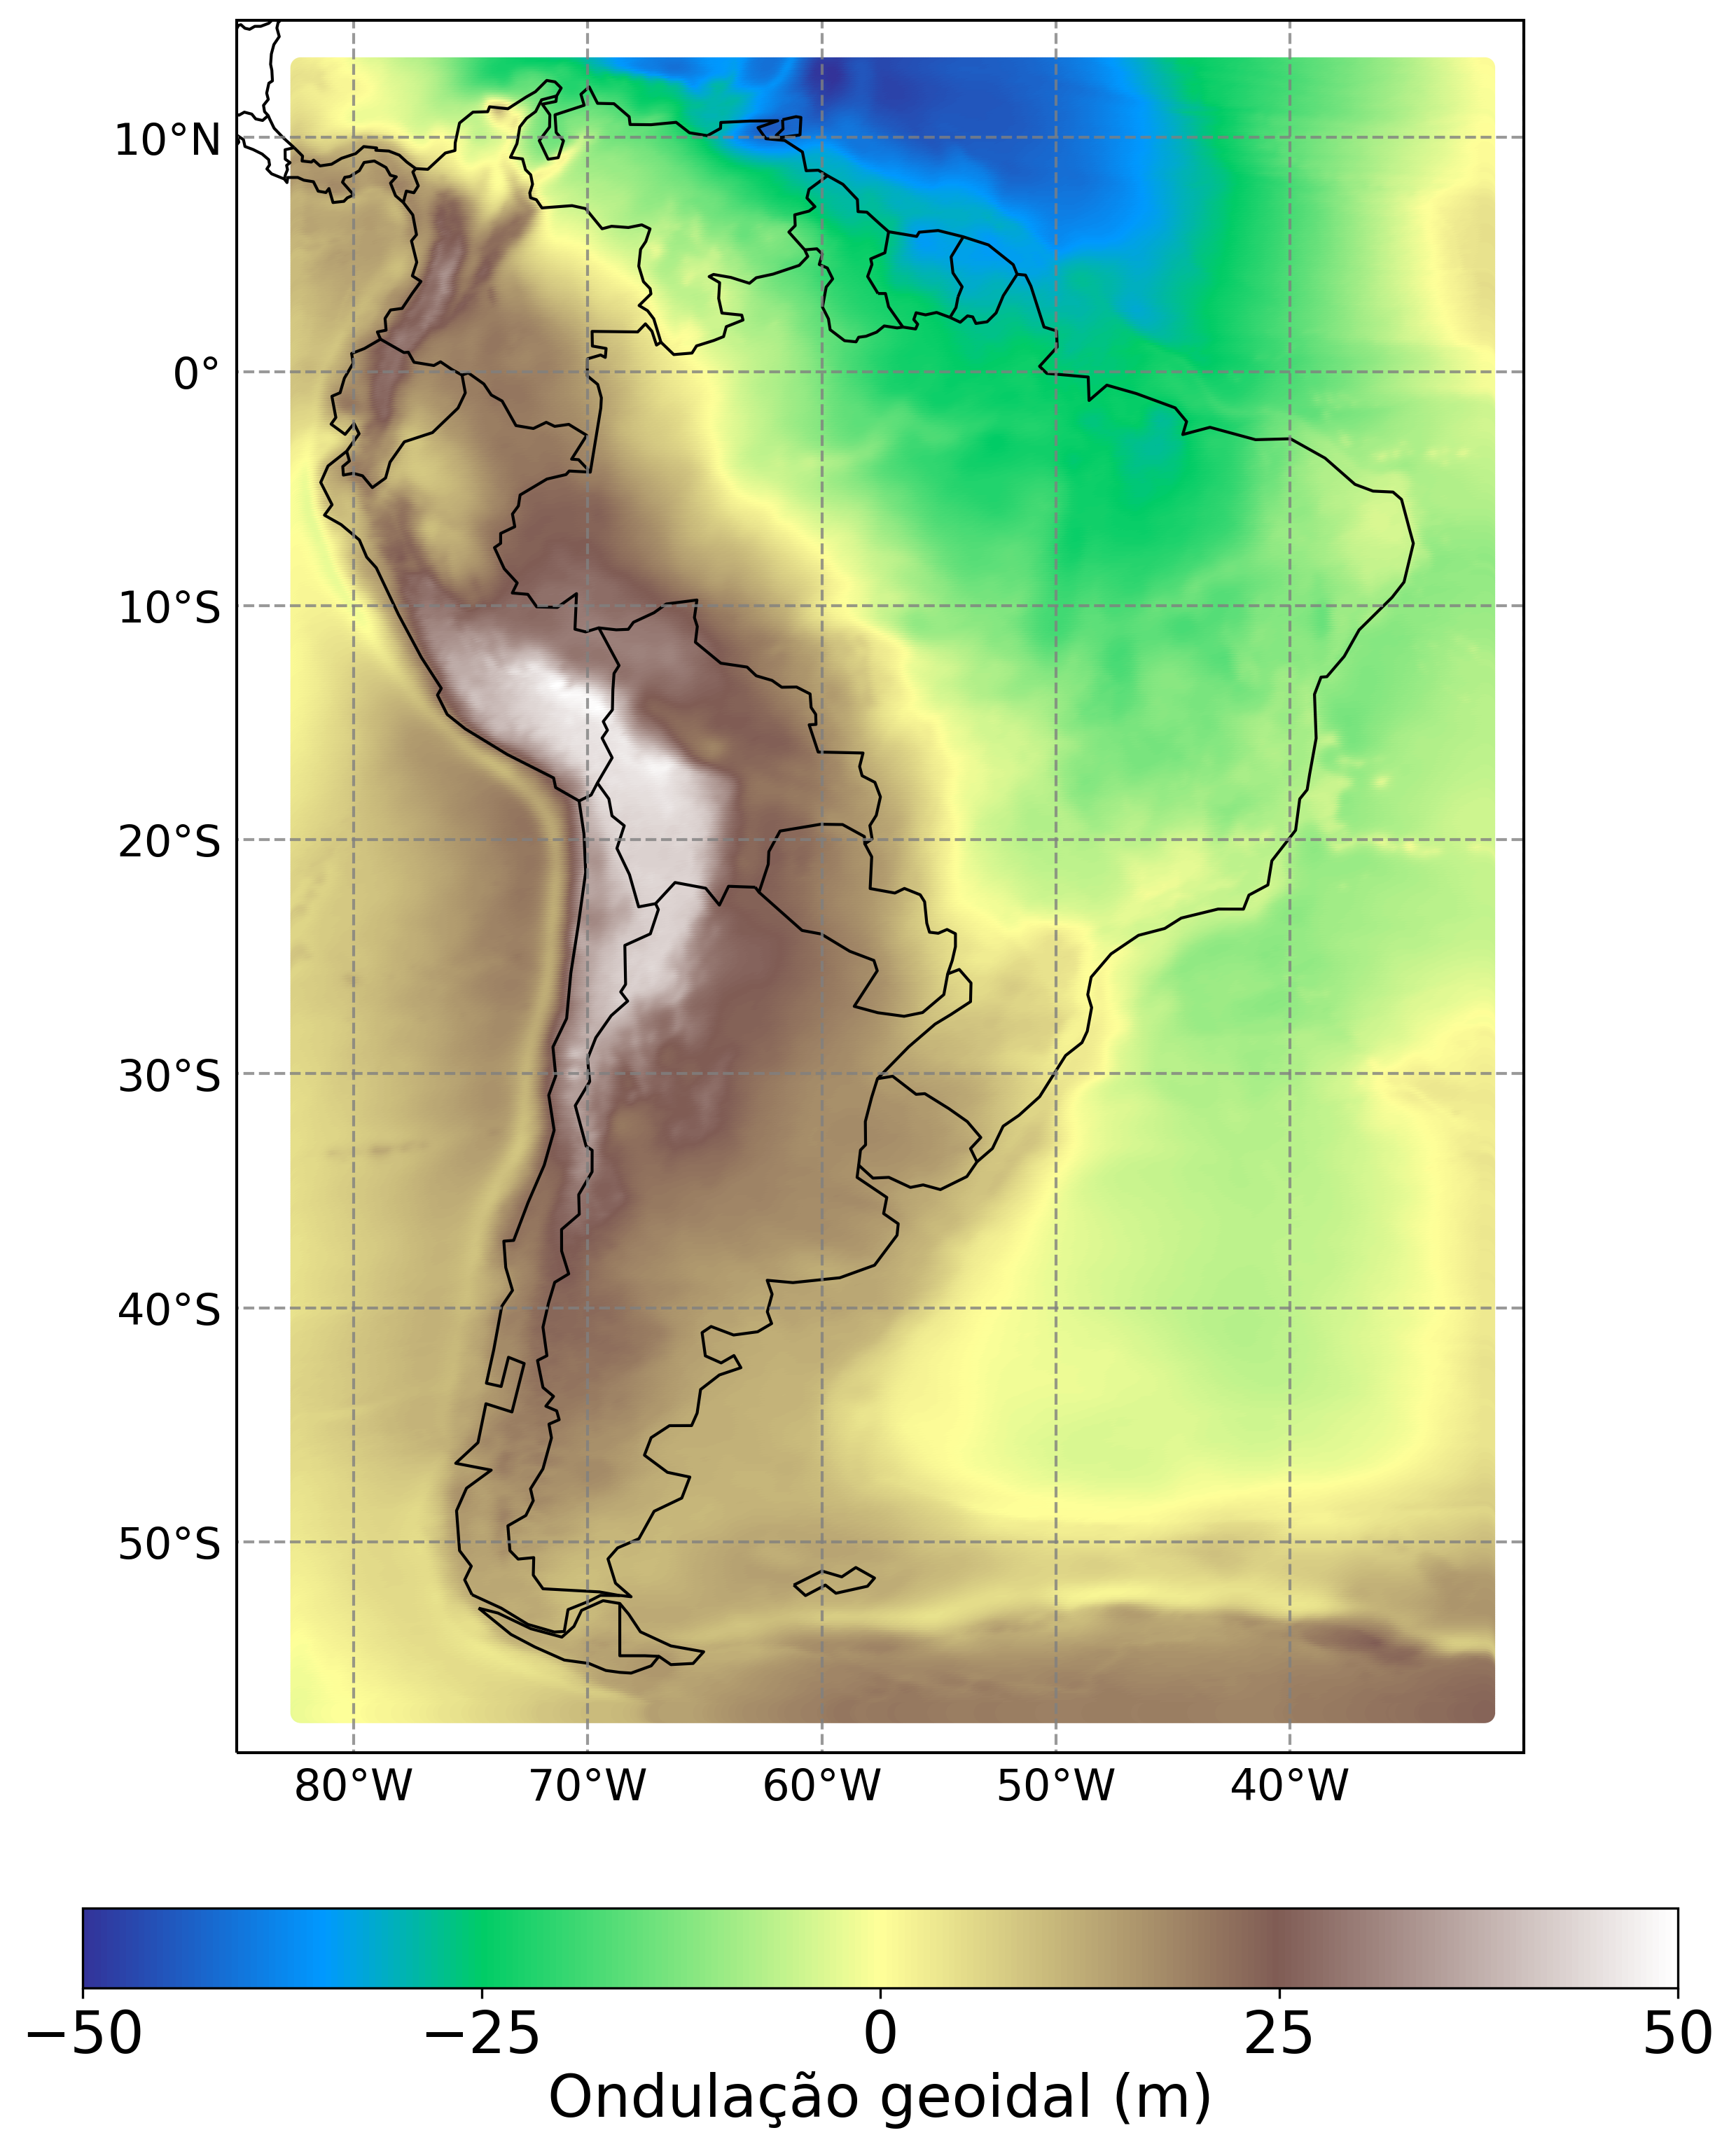
\includegraphics[scale=0.36]{figs/N_AS.png}}
	\caption{Mapas da anomalia de gravidade (a), distúrbio de gravidade (b), diferença entre distúrbio e anomalia de gravidade (c) e ondulação geoidal (d) sobre a América do Sul. Os contornos pretos representam os limites dos países.}  
	\label{subfig:anomalia}
\end{figure}